\documentclass[11pt]{article}
%\documentclass[dvips,11pt]{article}

% \usepackage{natbib}
% \setlength{\bibsep}{0pt plus 0.3ex}
\usepackage{titlesec}
\titlespacing*{\section}{0pt}{0.3\baselineskip}{0.3\baselineskip}
%,nohead,nofoot
%\usepackage[margin=1n,left=1cm,top=1cm,right=1.75cm,bottom=1.5cm]{geometry}
\usepackage[margin=1in,includeheadfoot,left=1cm,top=0.5cm,right=1.5cm,bottom=0.5cm]{geometry}
%\usepackage[margin=1in,includeheadfoot]{geometry}
\usepackage{url}
\usepackage{cite}
\usepackage{lipsum}
\usepackage{booktabs}
\usepackage{tabularx}

% ADD THE FOLLOWING COUPLE LINES INTO YOUR PREAMBLE
\let\OLDthebibliography\thebibliography
\renewcommand\thebibliography[1]{
  \OLDthebibliography{#1}
  \setlength{\parskip}{0pt}
  \setlength{\itemsep}{0pt plus 0.3ex}
}

\usepackage[pdftex]{graphicx}
\usepackage{url}
\usepackage{color}
\definecolor{darkred}{rgb}{0.5,0,0}
\definecolor{darkgreen}{rgb}{0,0.5,0}
\definecolor{darkblue}{rgb}{0,0,0.5}
%% macros
\newcommand{\ie}{i.e.}
\newcommand{\eg}{e.g.}
\newcommand{\Fix}[1]{\textbf{[[}{\color{red} #1}\textbf{]]}}
\newcommand{\Mar}[1]{\textbf{[[}{\color{blue} #1}\textbf{]]}}
\newcommand{\Comment}[1]{}

%% \setlength{\oddsidemargin}{0.25in}
%% \setlength{\textwidth}{6.5in}
%% \setlength{\topmargin}{0in}
%% \setlength{\textheight}{8.5in}

%\renewcommand\Affilfont{\fontsize{9}{10.8}\itshape}
% These force using more of the margins that is the default style

\begin{document}

\title{Finding Bugs in JavaScript Engines with Differential Testing}
\author{}
\date{}

% You can leave out "date" and it will be added automatically for today
% You can change the "\today" date to any text you like

\makeatletter
\def\maketitle{%
  \par{\centering\large\textbf{\@title}\normalsize\par}\vspace{3ex}%
  \par{\@author}%
  \par}
\makeatother

\maketitle

\vspace{-2ex}
\small    
\begin{table}[h!] 
  \centering%% Centro de Inform\'atica - CIn \\
  \begin{tabular*}{.85\linewidth}{l}

    Marcelo d'Amorim and Igor Sim\~oes (M.Sc. student)\\
    
    Postal Address: Av. Jornalista Anibal Fernandes, S/N. Cidade
    Universit\'aria, PE, Brazil, 50.740-560 \\
    
    Email addresses: \{damorim, isol2\}@cin.ufpe.br\\

    Phones: +55 (81) 2126-8430,
    ext. 4379 [work], +55 (81) 98800-2010 [mobile]\\

    Affiliation: Federal University of Pernambuco, Department of
    Computer Science\\

    Contact at Google:~Martin Barbella (mbarbella@google.com)

  \end{tabular*}
\end{table}
\normalsize

\vspace{-2ex}
\begin{abstract}
...
\end{abstract}

\section{Problem Space}

JavaScript (JS) is one of the most popular programming languages of
today~\cite{business-insider,stackify}. Its niche is front-end and
back-end web development\Comment{, supported several frameworks and
  runtimes (\eg{}, Express.js and Node.js)}. 

Engine implementations (\eg{}, Google's V8\Fix{cite}, Mozilla's
SpiderMonkey\Fix{cite}, and Microsoft's Chakra\Fix{cite}) need to
follow the constant changes in the language
specification~\cite{kangax}. Recently, the JavaScript
specification went through a bigger change compared to prior
releases\footnote{Called by the name of ECMAScript6
  (ES6)~\cite{es6-features}}. As in any piece of software, changes in
the specification often demand sensible changes in implementations
that could lead to errors, including regressions. In fact, bugs in JS
implementations are often reported by the general public, some of
which were reported by our team.

%% (confirmed by engine developers; see
%% Section~\ref{sec:results}) using a prototype of our solution (see
%% Section~\ref{sec:design}).

The lack of executable specifications that could be used as oracles is
an important obstacle for test generation--it prevents detection of
errors which are not explicit, like a crash.  The novelty of our
approach is the use of multiple engine implementations to assess input
validity and output correctness. \emph{Differential testing}\Fix{cite}
has been applied in a variety of contexts\Fix{cite cite}, but it has
not been used to find functional bugs in JS engines.

%\vspace{-1ex}
\begin{center}
\fbox{
  \begin{minipage}{11.75cm}
    \centering \textit{The goal of this project is to find bugs in
      implementations of JavaScript engines by leveraging diversity
      across implementations.}
  \end{minipage}
}
\end{center}
%\vspace{-1ex}

\section{Design Space}
\label{sec:design}

Fuzzing is a popular technique to generate new test inputs from
existing inputs\Fix{cite} with the typical goal of finding
crashes. Several fuzzing methods have been proposed in the past,
varying with respect to how new inputs are generated (\eg{},
mutation-based\Fix{cite}, grammar-based\Fix{cite}, and
random-based\Fix{cite}) and whether or not coverage information is
taken into account in the fuzzing process.


\begin{figure}[htbp]
  \centering
  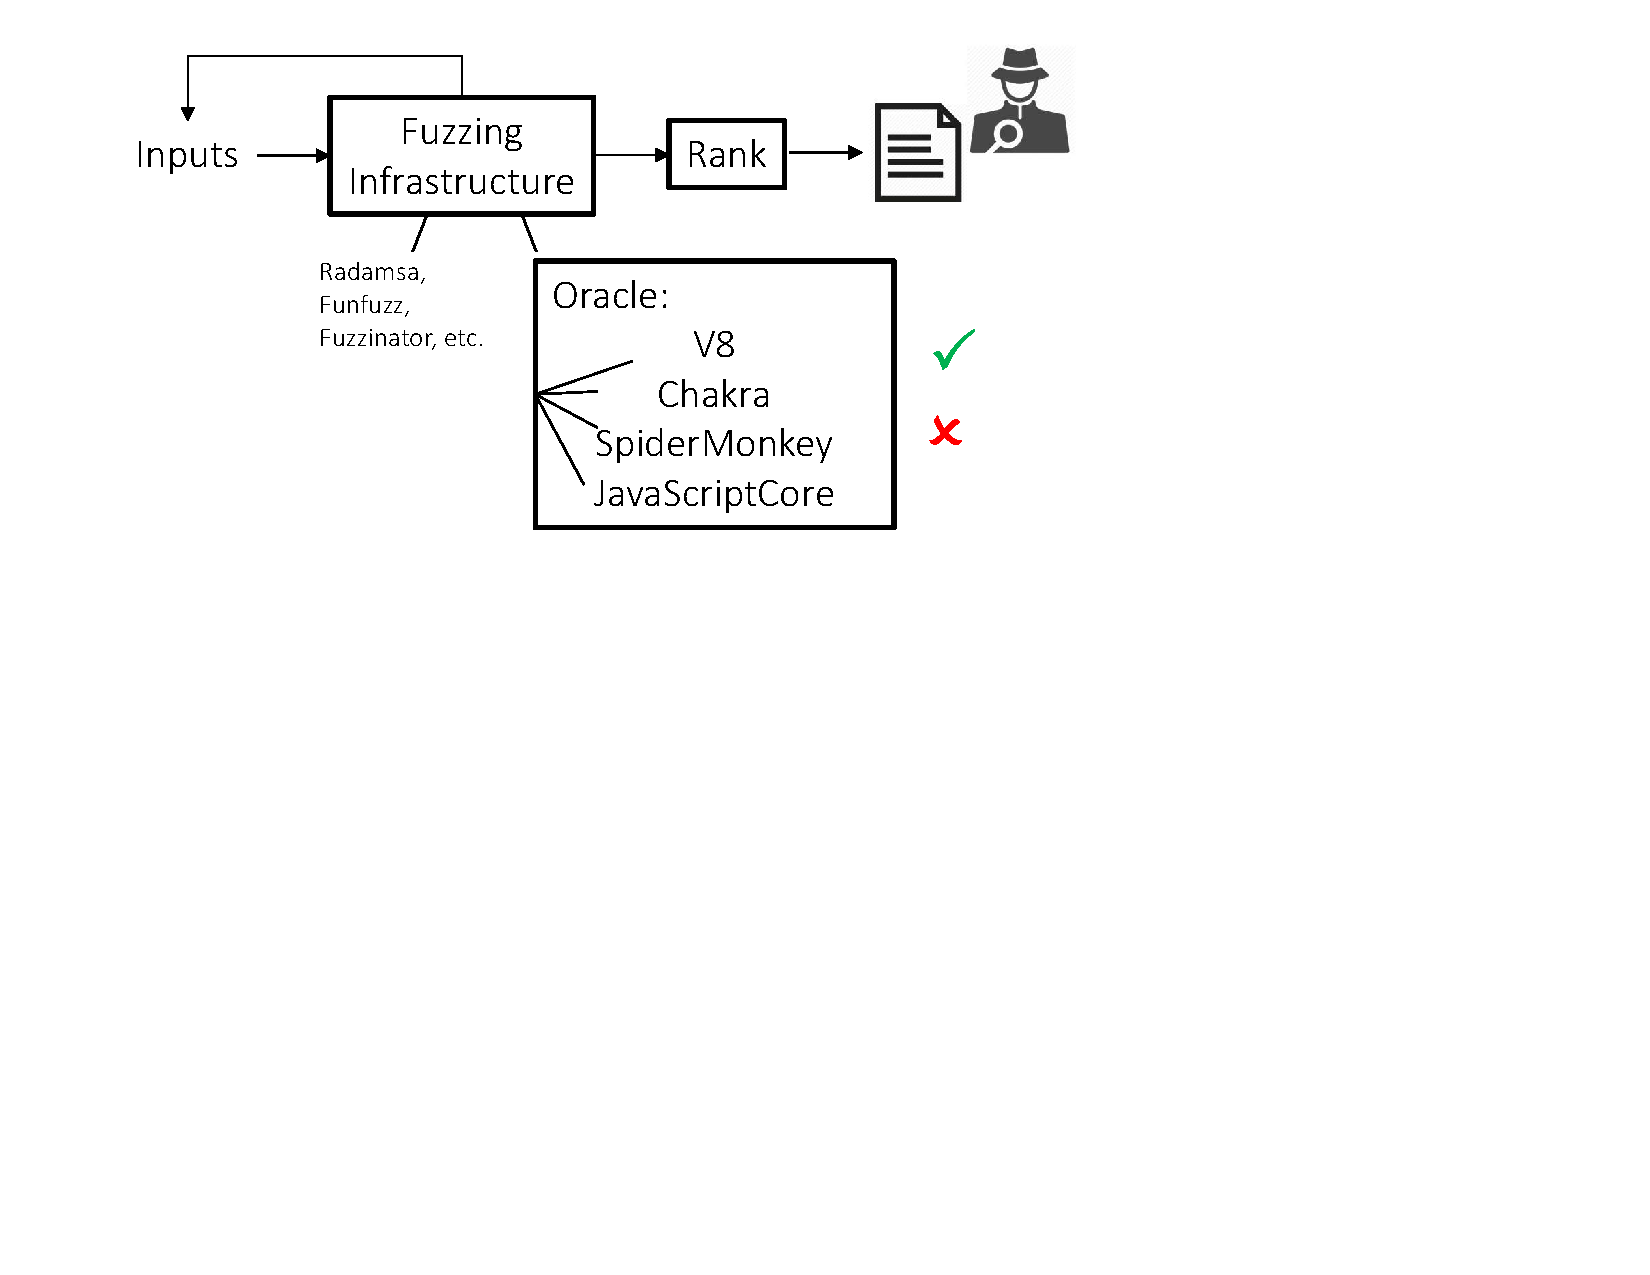
\includegraphics[trim=0 350 200 0,clip,width=0.5\textwidth]{google-awards-workflow}
  \label{fig:workflow}
  \caption{Workflow of Infrastructure.}
\end{figure}


\section{Related Work}

\Mar{rule of thumb: explain the
  contribution/novelty, then results achieved, and then how it relates
with our proposal.}
\Mar{this is not clear$\rightarrow$}Yang et al. \cite{yang-2011-finding} proposed CSmith\footnote{\url{http://embed.cs.utah.edu/csmith/}}, a grammar-fuzzer 
of C programs to generate invalid entries\Fix{the goal of a
  fuzzer is to generate valid inputs/entries. this is strange} and
find bugs in several C compilers\Fix{it is strange that you don't mention differential
  testing, which is central in CSmith, and the use of LLVM and GCC as
  oracles.}.\Mar{this is just listing fuzzers. don't do this. try to
  follow rule of thumb above.}Similar fuzzers involving grammar and rules are found in Holler et al. \cite{holler-2012-fuzzing} 
that exposes the LangFuzz to generate entries based in code fragments 
(language grammar, sample code, test suite) and the tool Mozilla 
Funfuzz\footnote{\url{https://github.com/MozillaSecurity/funfuzz}}
that implements a fuzzer based on JavaScript language to improve the 
testing for SpiderMonkey engine, the interpreter of Mozilla Firefox.
\Fix{...}



\vspace{1ex}\noindent\textbf{Input/Output.}~...

\section{Current Results}
\label{sec:results}

\Fix{list/describe/explain some of the bugs we found here}

\section{Data Policy}

The results produced with this research will be made available to the
public and to the research community.  All tools and data sets
developed will be available online, and the software will be released
under an open source license.


\footnotesize
\bibliographystyle{plain}
\bibliography{tmp}

\end{document}

